\documentclass[conference]{IEEEtran}
\IEEEoverridecommandlockouts
\usepackage[T1]{fontenc}
\usepackage{cite}
\usepackage{amsmath,amssymb}
\usepackage{graphicx}
\usepackage{booktabs}
\usepackage{xcolor}
\usepackage{tikz}
\usetikzlibrary{positioning,arrows.meta,fit}
\usepackage[hidelinks]{hyperref}

% ---------------------------------------------------------------------------------------------
% Every result number is a macro generated from the result files by scripts/make_tables.py.
% auto-generated by scripts/make_tables.py -- do not edit
\providecommand{\BenchCPU}{}\renewcommand{\BenchCPU}{AMD Ryzen 7 7730U}
\providecommand{\BenchThreads}{}\renewcommand{\BenchThreads}{8}
\providecommand{\FusExtraParams}{}\renewcommand{\FusExtraParams}{144}
\providecommand{\FusMs}{}\renewcommand{\FusMs}{37.1}
\providecommand{\LateMs}{}\renewcommand{\LateMs}{70.7}
\providecommand{\LumHi}{}\renewcommand{\LumHi}{--}
\providecommand{\LumLo}{}\renewcommand{\LumLo}{--}
\providecommand{\NSeeds}{}\renewcommand{\NSeeds}{--}
\providecommand{\NTest}{}\renewcommand{\NTest}{--}
\providecommand{\NTestBoxes}{}\renewcommand{\NTestBoxes}{--}
\providecommand{\NTestFrames}{}\renewcommand{\NTestFrames}{--}
\providecommand{\NTestPersons}{}\renewcommand{\NTestPersons}{--}
\providecommand{\NTrainBoxes}{}\renewcommand{\NTrainBoxes}{--}
\providecommand{\NTrainFrames}{}\renewcommand{\NTrainFrames}{--}
\providecommand{\NValBoxes}{}\renewcommand{\NValBoxes}{--}
\providecommand{\NValFrames}{}\renewcommand{\NValFrames}{--}
\providecommand{\NValScenes}{}\renewcommand{\NValScenes}{--}
\providecommand{\RDiffIrVsRgbApEst}{}\renewcommand{\RDiffIrVsRgbApEst}{--}
\providecommand{\RDiffIrVsRgbApFiftyEst}{}\renewcommand{\RDiffIrVsRgbApFiftyEst}{--}
\providecommand{\RDiffIrVsRgbApFiftyHi}{}\renewcommand{\RDiffIrVsRgbApFiftyHi}{--}
\providecommand{\RDiffIrVsRgbApFiftyLo}{}\renewcommand{\RDiffIrVsRgbApFiftyLo}{--}
\providecommand{\RDiffIrVsRgbApHi}{}\renewcommand{\RDiffIrVsRgbApHi}{--}
\providecommand{\RDiffIrVsRgbApLo}{}\renewcommand{\RDiffIrVsRgbApLo}{--}
\providecommand{\RDiffLateWbfVsIrApEst}{}\renewcommand{\RDiffLateWbfVsIrApEst}{--}
\providecommand{\RDiffLateWbfVsIrApFiftyEst}{}\renewcommand{\RDiffLateWbfVsIrApFiftyEst}{--}
\providecommand{\RDiffLateWbfVsIrApFiftyHi}{}\renewcommand{\RDiffLateWbfVsIrApFiftyHi}{--}
\providecommand{\RDiffLateWbfVsIrApFiftyLo}{}\renewcommand{\RDiffLateWbfVsIrApFiftyLo}{--}
\providecommand{\RDiffLateWbfVsIrApHi}{}\renewcommand{\RDiffLateWbfVsIrApHi}{--}
\providecommand{\RDiffLateWbfVsIrApLo}{}\renewcommand{\RDiffLateWbfVsIrApLo}{--}
\providecommand{\RDiffRgbVsGrayApEst}{}\renewcommand{\RDiffRgbVsGrayApEst}{--}
\providecommand{\RDiffRgbVsGrayApFiftyEst}{}\renewcommand{\RDiffRgbVsGrayApFiftyEst}{--}
\providecommand{\RDiffRgbVsGrayApFiftyHi}{}\renewcommand{\RDiffRgbVsGrayApFiftyHi}{--}
\providecommand{\RDiffRgbVsGrayApFiftyLo}{}\renewcommand{\RDiffRgbVsGrayApFiftyLo}{--}
\providecommand{\RDiffRgbVsGrayApHi}{}\renewcommand{\RDiffRgbVsGrayApHi}{--}
\providecommand{\RDiffRgbVsGrayApLo}{}\renewcommand{\RDiffRgbVsGrayApLo}{--}
\providecommand{\RDiffRgbtVsIrApEst}{}\renewcommand{\RDiffRgbtVsIrApEst}{--}
\providecommand{\RDiffRgbtVsIrApFiftyEst}{}\renewcommand{\RDiffRgbtVsIrApFiftyEst}{--}
\providecommand{\RDiffRgbtVsIrApFiftyHi}{}\renewcommand{\RDiffRgbtVsIrApFiftyHi}{--}
\providecommand{\RDiffRgbtVsIrApFiftyLo}{}\renewcommand{\RDiffRgbtVsIrApFiftyLo}{--}
\providecommand{\RDiffRgbtVsIrApHi}{}\renewcommand{\RDiffRgbtVsIrApHi}{--}
\providecommand{\RDiffRgbtVsIrApLo}{}\renewcommand{\RDiffRgbtVsIrApLo}{--}
\providecommand{\RDiffRgbtVsLateWbfApEst}{}\renewcommand{\RDiffRgbtVsLateWbfApEst}{--}
\providecommand{\RDiffRgbtVsLateWbfApFiftyEst}{}\renewcommand{\RDiffRgbtVsLateWbfApFiftyEst}{--}
\providecommand{\RDiffRgbtVsLateWbfApFiftyHi}{}\renewcommand{\RDiffRgbtVsLateWbfApFiftyHi}{--}
\providecommand{\RDiffRgbtVsLateWbfApFiftyLo}{}\renewcommand{\RDiffRgbtVsLateWbfApFiftyLo}{--}
\providecommand{\RDiffRgbtVsLateWbfApHi}{}\renewcommand{\RDiffRgbtVsLateWbfApHi}{--}
\providecommand{\RDiffRgbtVsLateWbfApLo}{}\renewcommand{\RDiffRgbtVsLateWbfApLo}{--}
\providecommand{\RDiffRgbtVsRgbApEst}{}\renewcommand{\RDiffRgbtVsRgbApEst}{--}
\providecommand{\RDiffRgbtVsRgbApFiftyEst}{}\renewcommand{\RDiffRgbtVsRgbApFiftyEst}{--}
\providecommand{\RDiffRgbtVsRgbApFiftyHi}{}\renewcommand{\RDiffRgbtVsRgbApFiftyHi}{--}
\providecommand{\RDiffRgbtVsRgbApFiftyLo}{}\renewcommand{\RDiffRgbtVsRgbApFiftyLo}{--}
\providecommand{\RDiffRgbtVsRgbApHi}{}\renewcommand{\RDiffRgbtVsRgbApHi}{--}
\providecommand{\RDiffRgbtVsRgbApLo}{}\renewcommand{\RDiffRgbtVsRgbApLo}{--}
\providecommand{\RDiffRgbtVsRgbtUnpairedApEst}{}\renewcommand{\RDiffRgbtVsRgbtUnpairedApEst}{--}
\providecommand{\RDiffRgbtVsRgbtUnpairedApFiftyEst}{}\renewcommand{\RDiffRgbtVsRgbtUnpairedApFiftyEst}{--}
\providecommand{\RDiffRgbtVsRgbtUnpairedApFiftyHi}{}\renewcommand{\RDiffRgbtVsRgbtUnpairedApFiftyHi}{--}
\providecommand{\RDiffRgbtVsRgbtUnpairedApFiftyLo}{}\renewcommand{\RDiffRgbtVsRgbtUnpairedApFiftyLo}{--}
\providecommand{\RDiffRgbtVsRgbtUnpairedApHi}{}\renewcommand{\RDiffRgbtVsRgbtUnpairedApHi}{--}
\providecommand{\RDiffRgbtVsRgbtUnpairedApLo}{}\renewcommand{\RDiffRgbtVsRgbtUnpairedApLo}{--}
\providecommand{\RGrayCleanAp}{}\renewcommand{\RGrayCleanAp}{--}
\providecommand{\RGrayCleanApFifty}{}\renewcommand{\RGrayCleanApFifty}{--}
\providecommand{\RGrayIrBlackoutApFifty}{}\renewcommand{\RGrayIrBlackoutApFifty}{--}
\providecommand{\RGrayIrNoiseApFifty}{}\renewcommand{\RGrayIrNoiseApFifty}{--}
\providecommand{\RGrayLumHighApFifty}{}\renewcommand{\RGrayLumHighApFifty}{--}
\providecommand{\RGrayLumLowApFifty}{}\renewcommand{\RGrayLumLowApFifty}{--}
\providecommand{\RGrayLumMidApFifty}{}\renewcommand{\RGrayLumMidApFifty}{--}
\providecommand{\RGrayRgbBlackoutApFifty}{}\renewcommand{\RGrayRgbBlackoutApFifty}{--}
\providecommand{\RGrayRgbFogApFifty}{}\renewcommand{\RGrayRgbFogApFifty}{--}
\providecommand{\RGrayRgbLowlightApFifty}{}\renewcommand{\RGrayRgbLowlightApFifty}{--}
\providecommand{\RGrayRgbNoiseApFifty}{}\renewcommand{\RGrayRgbNoiseApFifty}{--}
\providecommand{\RIrCleanAp}{}\renewcommand{\RIrCleanAp}{--}
\providecommand{\RIrCleanApFifty}{}\renewcommand{\RIrCleanApFifty}{--}
\providecommand{\RIrIrBlackoutApFifty}{}\renewcommand{\RIrIrBlackoutApFifty}{--}
\providecommand{\RIrIrNoiseApFifty}{}\renewcommand{\RIrIrNoiseApFifty}{--}
\providecommand{\RIrLumHighApFifty}{}\renewcommand{\RIrLumHighApFifty}{--}
\providecommand{\RIrLumLowApFifty}{}\renewcommand{\RIrLumLowApFifty}{--}
\providecommand{\RIrLumMidApFifty}{}\renewcommand{\RIrLumMidApFifty}{--}
\providecommand{\RIrRgbBlackoutApFifty}{}\renewcommand{\RIrRgbBlackoutApFifty}{--}
\providecommand{\RIrRgbFogApFifty}{}\renewcommand{\RIrRgbFogApFifty}{--}
\providecommand{\RIrRgbLowlightApFifty}{}\renewcommand{\RIrRgbLowlightApFifty}{--}
\providecommand{\RIrRgbNoiseApFifty}{}\renewcommand{\RIrRgbNoiseApFifty}{--}
\providecommand{\RIrShiftEightApFifty}{}\renewcommand{\RIrShiftEightApFifty}{--}
\providecommand{\RIrShiftFourApFifty}{}\renewcommand{\RIrShiftFourApFifty}{--}
\providecommand{\RIrShiftSixteenApFifty}{}\renewcommand{\RIrShiftSixteenApFifty}{--}
\providecommand{\RIrShiftThirtyTwoApFifty}{}\renewcommand{\RIrShiftThirtyTwoApFifty}{--}
\providecommand{\RIrShiftZeroApFifty}{}\renewcommand{\RIrShiftZeroApFifty}{--}
\providecommand{\RLateNmsCleanAp}{}\renewcommand{\RLateNmsCleanAp}{--}
\providecommand{\RLateNmsCleanApFifty}{}\renewcommand{\RLateNmsCleanApFifty}{--}
\providecommand{\RLateNmsIrBlackoutApFifty}{}\renewcommand{\RLateNmsIrBlackoutApFifty}{--}
\providecommand{\RLateNmsIrNoiseApFifty}{}\renewcommand{\RLateNmsIrNoiseApFifty}{--}
\providecommand{\RLateNmsLumHighApFifty}{}\renewcommand{\RLateNmsLumHighApFifty}{--}
\providecommand{\RLateNmsLumLowApFifty}{}\renewcommand{\RLateNmsLumLowApFifty}{--}
\providecommand{\RLateNmsLumMidApFifty}{}\renewcommand{\RLateNmsLumMidApFifty}{--}
\providecommand{\RLateNmsRgbBlackoutApFifty}{}\renewcommand{\RLateNmsRgbBlackoutApFifty}{--}
\providecommand{\RLateNmsRgbFogApFifty}{}\renewcommand{\RLateNmsRgbFogApFifty}{--}
\providecommand{\RLateNmsRgbLowlightApFifty}{}\renewcommand{\RLateNmsRgbLowlightApFifty}{--}
\providecommand{\RLateNmsRgbNoiseApFifty}{}\renewcommand{\RLateNmsRgbNoiseApFifty}{--}
\providecommand{\RLateWbfCleanAp}{}\renewcommand{\RLateWbfCleanAp}{--}
\providecommand{\RLateWbfCleanApFifty}{}\renewcommand{\RLateWbfCleanApFifty}{--}
\providecommand{\RLateWbfIrBlackoutApFifty}{}\renewcommand{\RLateWbfIrBlackoutApFifty}{--}
\providecommand{\RLateWbfIrNoiseApFifty}{}\renewcommand{\RLateWbfIrNoiseApFifty}{--}
\providecommand{\RLateWbfLumHighApFifty}{}\renewcommand{\RLateWbfLumHighApFifty}{--}
\providecommand{\RLateWbfLumLowApFifty}{}\renewcommand{\RLateWbfLumLowApFifty}{--}
\providecommand{\RLateWbfLumMidApFifty}{}\renewcommand{\RLateWbfLumMidApFifty}{--}
\providecommand{\RLateWbfRgbBlackoutApFifty}{}\renewcommand{\RLateWbfRgbBlackoutApFifty}{--}
\providecommand{\RLateWbfRgbFogApFifty}{}\renewcommand{\RLateWbfRgbFogApFifty}{--}
\providecommand{\RLateWbfRgbLowlightApFifty}{}\renewcommand{\RLateWbfRgbLowlightApFifty}{--}
\providecommand{\RLateWbfRgbNoiseApFifty}{}\renewcommand{\RLateWbfRgbNoiseApFifty}{--}
\providecommand{\RLateWbfShiftEightApFifty}{}\renewcommand{\RLateWbfShiftEightApFifty}{--}
\providecommand{\RLateWbfShiftFourApFifty}{}\renewcommand{\RLateWbfShiftFourApFifty}{--}
\providecommand{\RLateWbfShiftSixteenApFifty}{}\renewcommand{\RLateWbfShiftSixteenApFifty}{--}
\providecommand{\RLateWbfShiftThirtyTwoApFifty}{}\renewcommand{\RLateWbfShiftThirtyTwoApFifty}{--}
\providecommand{\RLateWbfShiftZeroApFifty}{}\renewcommand{\RLateWbfShiftZeroApFifty}{--}
\providecommand{\RRgbCleanAp}{}\renewcommand{\RRgbCleanAp}{--}
\providecommand{\RRgbCleanApFifty}{}\renewcommand{\RRgbCleanApFifty}{--}
\providecommand{\RRgbIrBlackoutApFifty}{}\renewcommand{\RRgbIrBlackoutApFifty}{--}
\providecommand{\RRgbIrNoiseApFifty}{}\renewcommand{\RRgbIrNoiseApFifty}{--}
\providecommand{\RRgbLumHighApFifty}{}\renewcommand{\RRgbLumHighApFifty}{--}
\providecommand{\RRgbLumLowApFifty}{}\renewcommand{\RRgbLumLowApFifty}{--}
\providecommand{\RRgbLumMidApFifty}{}\renewcommand{\RRgbLumMidApFifty}{--}
\providecommand{\RRgbRgbBlackoutApFifty}{}\renewcommand{\RRgbRgbBlackoutApFifty}{--}
\providecommand{\RRgbRgbFogApFifty}{}\renewcommand{\RRgbRgbFogApFifty}{--}
\providecommand{\RRgbRgbLowlightApFifty}{}\renewcommand{\RRgbRgbLowlightApFifty}{--}
\providecommand{\RRgbRgbNoiseApFifty}{}\renewcommand{\RRgbRgbNoiseApFifty}{--}
\providecommand{\RRgbShiftEightApFifty}{}\renewcommand{\RRgbShiftEightApFifty}{--}
\providecommand{\RRgbShiftFourApFifty}{}\renewcommand{\RRgbShiftFourApFifty}{--}
\providecommand{\RRgbShiftSixteenApFifty}{}\renewcommand{\RRgbShiftSixteenApFifty}{--}
\providecommand{\RRgbShiftThirtyTwoApFifty}{}\renewcommand{\RRgbShiftThirtyTwoApFifty}{--}
\providecommand{\RRgbShiftZeroApFifty}{}\renewcommand{\RRgbShiftZeroApFifty}{--}
\providecommand{\RRgbtCleanAp}{}\renewcommand{\RRgbtCleanAp}{--}
\providecommand{\RRgbtCleanApFifty}{}\renewcommand{\RRgbtCleanApFifty}{--}
\providecommand{\RRgbtIrBlackoutApFifty}{}\renewcommand{\RRgbtIrBlackoutApFifty}{--}
\providecommand{\RRgbtIrNoiseApFifty}{}\renewcommand{\RRgbtIrNoiseApFifty}{--}
\providecommand{\RRgbtLumHighApFifty}{}\renewcommand{\RRgbtLumHighApFifty}{--}
\providecommand{\RRgbtLumLowApFifty}{}\renewcommand{\RRgbtLumLowApFifty}{--}
\providecommand{\RRgbtLumMidApFifty}{}\renewcommand{\RRgbtLumMidApFifty}{--}
\providecommand{\RRgbtRgbBlackoutApFifty}{}\renewcommand{\RRgbtRgbBlackoutApFifty}{--}
\providecommand{\RRgbtRgbFogApFifty}{}\renewcommand{\RRgbtRgbFogApFifty}{--}
\providecommand{\RRgbtRgbLowlightApFifty}{}\renewcommand{\RRgbtRgbLowlightApFifty}{--}
\providecommand{\RRgbtRgbNoiseApFifty}{}\renewcommand{\RRgbtRgbNoiseApFifty}{--}
\providecommand{\RRgbtShiftEightApFifty}{}\renewcommand{\RRgbtShiftEightApFifty}{--}
\providecommand{\RRgbtShiftFourApFifty}{}\renewcommand{\RRgbtShiftFourApFifty}{--}
\providecommand{\RRgbtShiftSixteenApFifty}{}\renewcommand{\RRgbtShiftSixteenApFifty}{--}
\providecommand{\RRgbtShiftThirtyTwoApFifty}{}\renewcommand{\RRgbtShiftThirtyTwoApFifty}{--}
\providecommand{\RRgbtShiftZeroApFifty}{}\renewcommand{\RRgbtShiftZeroApFifty}{--}
\providecommand{\RRgbtUnpairedCleanAp}{}\renewcommand{\RRgbtUnpairedCleanAp}{--}
\providecommand{\RRgbtUnpairedCleanApFifty}{}\renewcommand{\RRgbtUnpairedCleanApFifty}{--}
\providecommand{\RRgbtUnpairedIrBlackoutApFifty}{}\renewcommand{\RRgbtUnpairedIrBlackoutApFifty}{--}
\providecommand{\RRgbtUnpairedIrNoiseApFifty}{}\renewcommand{\RRgbtUnpairedIrNoiseApFifty}{--}
\providecommand{\RRgbtUnpairedLumHighApFifty}{}\renewcommand{\RRgbtUnpairedLumHighApFifty}{--}
\providecommand{\RRgbtUnpairedLumLowApFifty}{}\renewcommand{\RRgbtUnpairedLumLowApFifty}{--}
\providecommand{\RRgbtUnpairedLumMidApFifty}{}\renewcommand{\RRgbtUnpairedLumMidApFifty}{--}
\providecommand{\RRgbtUnpairedRgbBlackoutApFifty}{}\renewcommand{\RRgbtUnpairedRgbBlackoutApFifty}{--}
\providecommand{\RRgbtUnpairedRgbFogApFifty}{}\renewcommand{\RRgbtUnpairedRgbFogApFifty}{--}
\providecommand{\RRgbtUnpairedRgbLowlightApFifty}{}\renewcommand{\RRgbtUnpairedRgbLowlightApFifty}{--}
\providecommand{\RRgbtUnpairedRgbNoiseApFifty}{}\renewcommand{\RRgbtUnpairedRgbNoiseApFifty}{--}
\providecommand{\RRgbtUnpairedShiftEightApFifty}{}\renewcommand{\RRgbtUnpairedShiftEightApFifty}{--}
\providecommand{\RRgbtUnpairedShiftFourApFifty}{}\renewcommand{\RRgbtUnpairedShiftFourApFifty}{--}
\providecommand{\RRgbtUnpairedShiftSixteenApFifty}{}\renewcommand{\RRgbtUnpairedShiftSixteenApFifty}{--}
\providecommand{\RRgbtUnpairedShiftThirtyTwoApFifty}{}\renewcommand{\RRgbtUnpairedShiftThirtyTwoApFifty}{--}
\providecommand{\RRgbtUnpairedShiftZeroApFifty}{}\renewcommand{\RRgbtUnpairedShiftZeroApFifty}{--}
\providecommand{\UniMs}{}\renewcommand{\UniMs}{35.4}

% Sentences whose *wording* depends on the direction of a result are wrapped in \pending{...}.
% They print in orange until the final results are in and the wording has been checked.
% Set \pendingfalse only after every \pending{} sentence has been verified against the tables.
\newif\ifpending \pendingtrue
\newcommand{\pending}[1]{\ifpending{\color{orange!85!black}#1}\else#1\fi}
% ---------------------------------------------------------------------------------------------

\begin{document}

\title{Visible, Thermal, or Both? A Controlled Study of Input Modality and Fusion for Lightweight All-Condition Person Detection}

\author{\IEEEauthorblockN{Utkarsh Tomar and Diya Khetan}
\IEEEauthorblockA{School of Computer Science and Engineering, Vellore Institute of Technology, Vellore 632014, Tamil Nadu, India\\
utkarsh.tomar2022@vitstudent.ac.in}}

\maketitle

\begin{abstract}
Surveillance cameras that must work around the clock are increasingly paired with long-wave infrared (LWIR) thermal sensors, but published comparisons of visible and thermal detectors often differ in dataset, scene and architecture at the same time, so the effect of the input modality itself is rarely isolated. We present a controlled study on the co-registered LLVIP benchmark in which five detectors share one architecture (YOLOv8n), one initialization and one training recipe, and differ only in their input: RGB, grayscale, thermal, early-fused RGB-T with correctly paired frames, and early-fused RGB-T whose thermal channel comes from an unrelated frame. We add a late-fusion ensemble of the RGB and thermal detectors and evaluate all systems over \NSeeds{} training seeds with paired bootstrap confidence intervals, across illumination levels, under synthetic sensor degradation and failure, and under controlled thermal-to-visible misregistration. On clean test data, AP$_{50}$ is \RRgbCleanApFifty\% for RGB, \RGrayCleanApFifty\% for grayscale, \RIrCleanApFifty\% for thermal and \RRgbtCleanApFifty\% for paired early fusion, whereas unpaired fusion reaches \RRgbtUnpairedCleanApFifty\%. \pending{Pairing, not the extra channel, is what makes fusion useful, and early fusion loses its advantage within a few pixels of misregistration, where late fusion degrades more gracefully.} Early fusion adds only \FusExtraParams{} parameters and runs at \FusMs{}\,ms per frame on a laptop CPU. All code, splits and per-run results are released.
\end{abstract}

\begin{IEEEkeywords}
multispectral object detection, thermal imaging, sensor fusion, surveillance, robustness, edge deployment
\end{IEEEkeywords}

% =============================================================================================
\section{Introduction}
Visible-spectrum (RGB) cameras are the default sensor for automated surveillance, perimeter security and driver assistance, but their images degrade quickly in darkness, glare, haze and smoke. LWIR thermal cameras image emitted heat rather than reflected light, so warm targets such as people remain visible at night~\cite{gade2014thermal,davis2005thermal}. Pairing the two sensors, and fusing them in a detector, has therefore become a standard route to all-condition detection~\cite{hwang2015kaist,liu2016multispectral,wagner2016fusion}.

Deciding \emph{whether} a second sensor is worth its cost requires knowing how much each modality contributes on its own, and this is where the evidence is weakest. Detectors for visible and thermal imagery are frequently trained on different datasets, captured from different viewpoints, containing different classes, and built on different architectures; any gap between them mixes the effect of the modality with the effect of everything else. Even within fusion papers, the unimodal baselines are often trained with a different recipe from the fused model. A second, less discussed confound is \emph{pairing}: a fused model can only exploit cross-spectral evidence if the two images show the same scene at the same instant and are spatially registered. Training on loosely associated or misaligned pairs is easy to do by accident, and a model trained that way can look like a fusion model while learning little from the second sensor.

This paper isolates these factors. Using the co-registered LLVIP dataset~\cite{jia2021llvip}, we derive five inputs from the same image pairs (Fig.~\ref{fig:design}) and train one lightweight detector per input with an identical recipe. Our contributions are:
\begin{enumerate}
\item A controlled comparison of RGB, grayscale, thermal and early-fused RGB-T inputs in which the architecture, initialization, recipe, data split and evaluation are held fixed, reported over multiple seeds with paired bootstrap confidence intervals.
\item A direct test of whether fusion benefits come from \emph{paired} information, obtained by training the same fusion model on deliberately unpaired thermal frames, together with a controlled misregistration sweep that compares early and late fusion.
\item An evaluation across measured scene illumination and under synthetic degradation or failure of either sensor, showing where each design fails.
\item Measured CPU cost of each design, and a complete release of code, data splits, per-run logs and result files, from which every number in this paper is generated automatically.
\end{enumerate}
We state the hypotheses before the results (Section~\ref{sec:hyp}) and report outcomes whether or not they support them.

% =============================================================================================
\section{Related Work}
\textbf{Thermal and multispectral pedestrian detection.} Early thermal detectors relied on hand-designed templates~\cite{davis2005thermal}. The KAIST benchmark~\cite{hwang2015kaist} introduced aligned visible--thermal video for pedestrian detection and made multispectral fusion a mainstream topic. LLVIP~\cite{jia2021llvip} provides strictly registered visible--infrared pairs captured mostly in low light, and M$^3$FD~\cite{liu2022tardal} extends paired data to several object classes.

\textbf{Where to fuse.} Fusion can happen at the input (early), in intermediate feature maps (halfway), or at the level of detections (late). Liu \emph{et al.}~\cite{liu2016multispectral} and Wagner \emph{et al.}~\cite{wagner2016fusion} compared these stages for CNN detectors and found halfway fusion strongest on KAIST; K\"onig \emph{et al.}~\cite{konig2017rpn} fused inside a region-proposal network. Later work weights the modalities by predicted illumination~\cite{li2019iafrcnn,guan2019illumination}, by attention~\cite{zhang2021gaff}, by modality imbalance~\cite{zhou2020mbnet} or by uncertainty~\cite{kim2022uncertainty}. Late fusion of independently trained detectors, for example by probabilistic ensembling~\cite{chen2022proben} or weighted box fusion~\cite{solovyev2021wbf}, needs no paired training data and tolerates some misregistration.

\textbf{Alignment.} Even datasets advertised as aligned contain residual offsets between modalities; Zhang \emph{et al.}~\cite{zhang2019arcnn} showed that this weak alignment harms fusion and proposed a region-alignment module. We complement such architectural fixes with a controlled measurement of how quickly a simple fusion detector degrades as registration worsens.

\textbf{Efficient detectors.} One-stage YOLO-family detectors~\cite{redmon2016yolo,jocher2023yolov8} and real-time transformer detectors~\cite{carion2020detr,zhao2024rtdetr} dominate deployment on constrained hardware. We use the smallest YOLOv8 variant because it is a common edge baseline and because a 4-channel input changes it by only one convolution.

% =============================================================================================
\section{Study Design}

\begin{figure}[t]
\centering
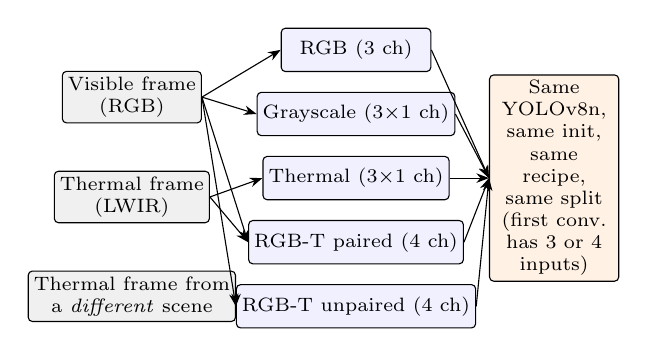
\begin{tikzpicture}[font=\scriptsize, node distance=2.5mm and 3mm,
  box/.style={draw, rounded corners=1.5pt, align=center, minimum height=5.5mm, inner sep=2pt},
  src/.style={box, fill=gray!12}, var/.style={box, fill=blue!6, minimum width=19mm}, arr/.style={-{Stealth[length=1.6mm]}, thin}]
\node[src] (rgb) {Visible frame\\(RGB)};
\node[src, below=6mm of rgb] (ir) {Thermal frame\\(LWIR)};
\node[src, below=6mm of ir] (irx) {Thermal frame from\\a \emph{different} scene};
\node[var, right=10mm of rgb, yshift=6mm] (v1) {RGB (3 ch)};
\node[var, below=of v1] (v2) {Grayscale (3$\times$1 ch)};
\node[var, below=of v2] (v3) {Thermal (3$\times$1 ch)};
\node[var, below=of v3] (v4) {RGB-T paired (4 ch)};
\node[var, below=of v4] (v5) {RGB-T unpaired (4 ch)};
\draw[arr] (rgb.east) -- (v1.west); \draw[arr] (rgb.east) -- (v2.west); \draw[arr] (rgb.east) -- (v4.west); \draw[arr] (rgb.east) -- (v5.west);
\draw[arr] (ir.east) -- (v3.west); \draw[arr] (ir.east) -- (v4.west);
\draw[arr] (irx.east) -- (v5.west);
\node[box, right=5mm of v3, fill=orange!10, minimum height=26mm, text width=15mm] (det) {Same YOLOv8n,\\same init,\\same recipe,\\same split\\(first conv.\\has 3 or 4\\inputs)};
\foreach \v in {v1,v2,v3,v4,v5} \draw[arr] (\v.east) -- (det.west);
\end{tikzpicture}
\caption{Study design. Five inputs are derived from the same co-registered LLVIP pairs; only the input differs between detectors. The RGB and thermal detectors are also combined by late fusion.}
\label{fig:design}
\end{figure}

\subsection{Data}
LLVIP~\cite{jia2021llvip} contains 15{,}488 visible--infrared image pairs of pedestrians at $1280\times1024$, registered by the dataset authors and annotated with one shared set of person boxes; most frames were captured in low light. We use the official test split (\NTestFrames{} frames, \NTestBoxes{} persons). Because LLVIP has no validation split, we hold out \NValScenes{} complete scenes of the official training set (\NValFrames{} frames) for model selection and train on the remaining \NTrainFrames{} frames; holding out whole scenes prevents near-duplicate consecutive frames from leaking between training and validation. All images are resized once to $640\times512$, which is exactly the resolution the detector sees at an input size of 640, and stored losslessly.

\textbf{Inputs.} From each registered pair we build: \emph{RGB}; \emph{grayscale} (ITU-R BT.601 luma of the RGB image, replicated to three channels); \emph{thermal} (the LWIR image replicated to three channels); \emph{RGB-T paired}, a 4-channel image $[R,G,B,T]$; and \emph{RGB-T unpaired}, identical except that the thermal channel of every training and validation frame is replaced by the thermal image of a randomly chosen frame from a different scene. The unpaired model is always tested on correctly paired frames. It reproduces, under control, the situation of a ``fusion'' model trained on sensor streams that are not associated, and it separates two explanations for a fusion gain: extra input capacity, or cross-spectral evidence about the same object.

\subsection{Detectors and training}
All detectors are YOLOv8n~\cite{jocher2023yolov8} (3.0\,M parameters): a CSP-style backbone with C2f blocks, a PAN feature pyramid and an anchor-free decoupled head, with one output class. Each is initialized from the same COCO-pretrained weights~\cite{lin2014coco}. For 4-channel inputs, the first convolution receives the pretrained RGB filters on the RGB channels and their mean on the thermal channel, and all four are scaled by $3/4$ so that the expected pre-normalization response matches the pretrained model; the remaining 144 new weights are the only architectural difference.

Every run uses the same recipe: 20 epochs, input size 640, batch 16, SGD (momentum 0.937, weight decay $5\times10^{-4}$) with learning rate 0.01, 3 warm-up epochs and cosine decay, mosaic augmentation (disabled for the last 5 epochs), random scaling ($\pm$50\%), translation (10\%) and horizontal flipping, automatic mixed precision, and no early stopping. HSV colour jitter is disabled for \emph{all} runs, because it cannot be applied to 4-channel inputs and leaving it on for the 3-channel runs would confound the comparison. The checkpoint with the best validation mAP is kept. We train \NSeeds{} seeds per input on one NVIDIA T4 GPU.

\textbf{Late fusion.} The RGB and thermal detectors of the same seed are run independently and their detections are merged, either by weighted box fusion (WBF)~\cite{solovyev2021wbf} (IoU 0.55, equal weights, scores averaged over the two detectors so that single-sensor detections are down-weighted) or by pooling both sets and applying non-maximum suppression (IoU 0.7).

\subsection{Evaluation}
We report COCO-style average precision~\cite{lin2014coco} for the person class: AP$_{50}$, AP$_{75}$ and AP (averaged over IoU 0.50:0.05:0.95), with at most 100 detections per image, computed with our own implementation, which agrees with \texttt{pycocotools} to machine precision on the same detections. All detectors use a confidence threshold of 0.001, NMS IoU 0.7 and input size 640. Results are the mean and standard deviation over seeds. Confidence intervals come from a paired image-level bootstrap~\cite{efron1994bootstrap} with 1{,}000 resamples, drawing the same resampled images for all systems, so differences between systems are paired.

\textbf{Illumination.} LLVIP has no day/night label, so we measure illumination directly: the mean luma of each visible test image. We split the test set into terciles of this value (thresholds \LumLo{} and \LumHi{} on a 0--255 scale).

\textbf{Sensor degradation.} We apply fixed, seeded perturbations to one sensor at test time: for the visible camera, \emph{low light} (gamma 2.2, gain 0.4, Gaussian read noise $\sigma{=}6$), \emph{fog} (atmospheric scattering model with constant transmission 0.45 and airlight 0.8), \emph{noise} (Gaussian, $\sigma{=}25$) and \emph{off} (all zeros); for the thermal camera, \emph{noise} ($\sigma{=}25$) and \emph{off}. The perturbations follow the spirit of common-corruption benchmarks~\cite{hendrycks2019corruptions} and are applied identically to every system. They are image-level simulations: the fog model, for instance, attenuates only the visible image and does not model LWIR attenuation, so these results measure how each design reacts when one input degrades, not the physics of any particular weather.

\textbf{Misregistration.} We shift the thermal image horizontally by $k\in\{4,8,16,32\}$ pixels at working resolution ($8$--$64$ pixels at native resolution) while keeping the RGB image and the labels fixed.

\subsection{Hypotheses}\label{sec:hyp}
We fixed the following hypotheses before training any model:
\textbf{H1} Colour helps: RGB $>$ grayscale.
\textbf{H2} Thermal outperforms RGB on LLVIP, with the largest gap in the darkest tercile.
\textbf{H3} Paired early fusion outperforms the best single modality.
\textbf{H4} Unpaired fusion does not outperform the best single modality, i.e.\ the gain in H3 requires pairing.
\textbf{H5} When one sensor fails, fusion degrades towards the surviving modality rather than collapsing.
\textbf{H6} Early fusion is more sensitive to misregistration than late fusion.

% =============================================================================================
\section{Results}

\begin{table}[t]\centering\caption{Detection on the LLVIP test set (clean inputs). Mean$\pm$std over \NSeeds{} seeds; 95\% CI from a paired image-level bootstrap.}\label{tab:main}
\setlength{\tabcolsep}{3pt}\footnotesize
\begin{tabular}{@{}lccccc@{}}\toprule
Input & Ch. & AP$_{50}$ & 95\% CI & AP$_{75}$ & AP \\ \midrule
RGB & 3 & -- & -- & -- & -- \\
Grayscale & 3$^\dagger$ & -- & -- & -- & -- \\
Thermal (LWIR) & 3$^\dagger$ & -- & -- & -- & -- \\
Early fusion (RGB-T, paired) & 4 & -- & -- & -- & -- \\
Early fusion (RGB-T, unpaired) & 4 & -- & -- & -- & -- \\
Late fusion (WBF) & 3+3 & -- & -- & -- & -- \\
Late fusion (NMS) & 3+3 & -- & -- & -- & -- \\
\bottomrule\end{tabular}
\\[2pt]{\scriptsize $^\dagger$single-channel image replicated to 3 channels.}
\end{table}


\subsection{Effect of input modality (H1--H3)}
Table~\ref{tab:main} gives the clean test results. Below, $\Delta$ denotes a difference in AP$_{50}$ points between seed-averaged systems, with the 95\% CI of the paired bootstrap. \pending{Removing colour costs accuracy: RGB$-$grayscale $\Delta={}$\RDiffRgbVsGrayApFiftyEst{} [\RDiffRgbVsGrayApFiftyLo, \RDiffRgbVsGrayApFiftyHi] (H1).} \pending{Thermal is the strongest single modality: thermal$-$RGB $\Delta={}$\RDiffIrVsRgbApFiftyEst{} [\RDiffIrVsRgbApFiftyLo, \RDiffIrVsRgbApFiftyHi] (H2).} \pending{Paired early fusion improves on thermal alone: $\Delta={}$\RDiffRgbtVsIrApFiftyEst{} [\RDiffRgbtVsIrApFiftyLo, \RDiffRgbtVsIrApFiftyHi] (H3), and on late fusion by WBF: $\Delta={}$\RDiffRgbtVsLateWbfApFiftyEst{} [\RDiffRgbtVsLateWbfApFiftyLo, \RDiffRgbtVsLateWbfApFiftyHi].}

\begin{table}[t]\centering\caption{AP$_{50}$ by scene illumination (terciles of mean visible-image luma; thresholds \LumLo{} and \LumHi{} on a 0--255 scale; $n$ = -- / -- / -- images).}\label{tab:illum}
\footnotesize
\begin{tabular}{@{}lccc@{}}\toprule
Input & Darkest & Middle & Brightest \\ \midrule
RGB & -- & -- & -- \\
Grayscale & -- & -- & -- \\
Thermal (LWIR) & -- & -- & -- \\
Early fusion (RGB-T, paired) & -- & -- & -- \\
Early fusion (RGB-T, unpaired) & -- & -- & -- \\
Late fusion (WBF) & -- & -- & -- \\
Late fusion (NMS) & -- & -- & -- \\
\bottomrule\end{tabular}
\end{table}


\subsection{Effect of illumination}
Table~\ref{tab:illum} splits the test set by measured brightness. \pending{The RGB detector falls from \RRgbLumHighApFifty\% AP$_{50}$ in the brightest tercile to \RRgbLumLowApFifty\% in the darkest, whereas thermal remains between \RIrLumLowApFifty\% and \RIrLumHighApFifty\%, so the RGB--thermal gap is largest in the dark (H2).} Because LLVIP is predominantly a low-light dataset, even its ``brightest'' tercile is dusk or artificially lit night scenery; these terciles are not a day/night split, and daylight performance should not be extrapolated from them.

\subsection{Does fusion need pairing? (H4, H6)}
\pending{Trained on unpaired frames, the fusion model reaches \RRgbtUnpairedCleanApFifty\% AP$_{50}$ on paired test data; paired$-$unpaired $\Delta={}$\RDiffRgbtVsRgbtUnpairedApFiftyEst{} [\RDiffRgbtVsRgbtUnpairedApFiftyLo, \RDiffRgbtVsRgbtUnpairedApFiftyHi] (H4).} The same architecture and input capacity therefore do not suffice: the benefit of the extra channel comes from the correspondence between the two images.

\begin{figure}[t]
\centering
\includegraphics[width=\columnwidth]{generated/fig_misalign.pdf}
\caption{AP$_{50}$ as the thermal image is shifted relative to the visible image and the labels (mean$\pm$std over seeds). The RGB-only detector does not use the thermal image and is shown for reference.}
\label{fig:misalign}
\end{figure}

Fig.~\ref{fig:misalign} shows the effect of misregistration. \pending{Paired early fusion drops from \RRgbtShiftZeroApFifty\% to \RRgbtShiftEightApFifty\% at an 8-pixel offset (16\,px native) and to \RRgbtShiftThirtyTwoApFifty\% at 32\,px, while late fusion drops from \RLateWbfShiftZeroApFifty\% to \RLateWbfShiftThirtyTwoApFifty\% (H6).} Because the labels follow the visible image, the thermal-only detector also loses accuracy as its image moves away from the boxes; this curve measures the localization error that a misregistered thermal sensor induces, and it bounds how much of the degradation is due to the fusion model itself.

\begin{table*}[t]\centering\caption{AP$_{50}$ under synthetic test-time degradation of one sensor (mean over seeds). A model is only affected by degradations of the sensors it uses.}\label{tab:robust}
\footnotesize
\begin{tabular}{@{}lccccccc@{}}\toprule
& & \multicolumn{4}{c}{Visible camera degraded} & \multicolumn{2}{c}{Thermal camera degraded} \\ \cmidrule(lr){3-6}\cmidrule(lr){7-8}
Input & Clean & Low-light & Fog & Noise & Off & Noise & Off \\ \midrule
RGB & -- & -- & -- & -- & -- & -- & -- \\
Grayscale & -- & -- & -- & -- & -- & -- & -- \\
Thermal (LWIR) & -- & -- & -- & -- & -- & -- & -- \\
Early fusion (RGB-T, paired) & -- & -- & -- & -- & -- & -- & -- \\
Early fusion (RGB-T, unpaired) & -- & -- & -- & -- & -- & -- & -- \\
Late fusion (WBF) & -- & -- & -- & -- & -- & -- & -- \\
Late fusion (NMS) & -- & -- & -- & -- & -- & -- & -- \\
\bottomrule\end{tabular}
\end{table*}


\subsection{Sensor degradation and failure (H5)}
Table~\ref{tab:robust} reports AP$_{50}$ when one sensor is degraded. \pending{When the visible camera is switched off, paired early fusion retains \RRgbtRgbBlackoutApFifty\% AP$_{50}$ against \RIrCleanApFifty\% for the thermal-only detector, and when the thermal camera is switched off it retains \RRgbtIrBlackoutApFifty\% against \RRgbCleanApFifty\% for RGB (H5).} \pending{Late fusion degrades to its surviving detector by construction, which makes it the more predictable design under sensor failure.} Early fusion was never trained with a missing modality; modality dropout during training is a simple remedy that we leave to future work.

\begin{table}[t]\centering\caption{Cost of each design on a laptop CPU (\BenchCPU{}, batch 1, 640$\times$512 input, FP32, median of 100 runs).}\label{tab:eff}
\setlength{\tabcolsep}{2.5pt}\footnotesize
\begin{tabular}{@{}lcccccc@{}}\toprule
& Params & & \multicolumn{2}{c}{Latency (ms)} & & ONNX \\ \cmidrule(lr){4-5}
Model & (M) & GFLOPs & PyTorch & ORT & FPS & (MB) \\ \midrule
Unimodal & 3.006 & 6.47 & 58.1 & 35.4 & 28 & 11.7 \\
Early fusion & 3.006 & 6.49 & 65.3 & 37.1 & 27 & 11.7 \\
Late fusion$^\ast$ &6.012 & 12.93 & -- & 70.7 & 14 & 23.3 \\
\bottomrule\end{tabular}
\\[2pt]{\scriptsize $^\ast$two unimodal detectors run sequentially; box-fusion time excluded.}
\end{table}


\subsection{Computational cost}
Table~\ref{tab:eff} lists the measured cost on a laptop CPU (\BenchCPU, \BenchThreads{} PyTorch threads, ONNX Runtime 1.30). Early fusion adds \FusExtraParams{} parameters and $<$1\% of the FLOPs of the unimodal detector and runs in \FusMs{}\,ms versus \UniMs{}\,ms per frame. Late fusion runs two detectors, roughly doubling latency (\LateMs{}\,ms before box fusion). All three designs run faster than 10 frames per second on this CPU without a GPU.

% =============================================================================================
\section{Discussion and Limitations}
\pending{Three practical conclusions follow. First, on low-light data a thermal detector alone recovers most of the achievable accuracy, and adding colour to a thermal detector helps only if the frames are truly paired and registered. Second, the unpaired-fusion result is a warning for system builders: a pipeline that pairs frames loosely, for example by index across two independently recorded streams, produces a model that looks multimodal but gains nothing from the second sensor. Third, early fusion is the cheapest design but is the most fragile to misregistration and to sensor failure, whereas late fusion costs a second detector but degrades gracefully; which trade-off is right depends on how well the sensors can be calibrated in the field.}

\textbf{Limitations.} (i) LLVIP contains one class (person), fixed surveillance viewpoints and mostly low-light scenes; conclusions about daylight, vehicles or aerial viewpoints need other paired datasets such as M$^3$FD~\cite{liu2022tardal}. (ii) We study one lightweight architecture and one short training schedule; larger models or halfway (feature-level) fusion~\cite{liu2016multispectral,zhang2021gaff} may change the size of the effects. (iii) Degradations are synthetic and applied to one sensor at a time; real fog, smoke and rain also affect LWIR imagery, and real sensor noise is not Gaussian. (iv) Misregistration is simulated as a global horizontal shift, whereas real parallax varies with depth. (v) Our illumination terciles are a proxy for lighting conditions and are confined to the range of LLVIP.

\textbf{Relation to defence surveillance.} Perimeter security and force protection are important motivating applications for all-condition detection. Our experiments use civilian pedestrian data only, and we make no claim about the detection of vehicles, equipment or camouflaged targets, which would require paired data containing such objects.

% =============================================================================================
\section{Conclusion}
Holding the architecture, recipe and data fixed, and changing only the input, we measured the contribution of colour, thermal imagery, pairing and registration to lightweight person detection on LLVIP. \pending{Thermal input dominates in low light, paired early fusion adds a further gain at almost no cost, and that gain disappears when the thermal frames are unpaired and shrinks quickly with misregistration.} We release the complete pipeline so that the same controlled protocol can be applied to other paired datasets and fusion architectures.

\section*{Code and Data Availability}
Code, the scene-level validation split, training logs, trained weights and all result files are available at \url{https://github.com/utkarsht123/Military-Asset-Detection-} (folder \texttt{esci2027}). LLVIP is available from its authors under its own terms of use~\cite{jia2021llvip}.

\bibliographystyle{IEEEtran}
\bibliography{refs}

\end{document}
